%%%%%%%%%%%%%%%%%%%%%%%%%%%%%%%%%%%%%%%%%
% Beamer Presentation
% LaTeX Template
% Version 1.0 (10/11/12)
%
% This template has been downloaded from:
% http://www.LaTeXTemplates.com
%
% License:
% CC BY-NC-SA 3.0 (http://creativecommons.org/licenses/by-nc-sa/3.0/)
%
%%%%%%%%%%%%%%%%%%%%%%%%%%%%%%%%%%%%%%%%%

%----------------------------------------------------------------------------------------
%	PACKAGES AND THEMES
%----------------------------------------------------------------------------------------

\documentclass[xcolor=dvipsnames]{beamer}
\usepackage{tikz}
\usepackage{graphicx}
\usepackage{setspace}
\usepackage{fancyvrb}
\usepackage{lipsum}
\usepackage{verbatimbox}
\setbeamertemplate{background canvas}{
\begin{tikzpicture}
\node[opacity=.15]{
\hspace{3cm}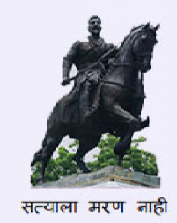
\includegraphics[height=0.8\paperheight]{logo.png}
};
\end{tikzpicture}}

\mode<presentation> {

% The Beamer class comes with a number of default slide themes
% which change the colors and layouts of slides. Below this is a list
% of all the themes, uncomment each in turn to see what they look like.
\usefonttheme[stillsansseriftext]{structurebold}

%\usetheme{default}
\usetheme{AnnArbor}
%\usetheme{Antibes}
%\usetheme{Bergen}
%\usetheme{Berkeley}
%\usetheme{Berlin}
%\usetheme{Boadilla}
%\usetheme{CambridgeUS}
%\usetheme{Copenhagen}
%\usetheme{Darmstadt}
%\usetheme{Dresden}
%\usetheme{Frankfurt}
%\usetheme{Goettingen}
%\usetheme{Hannover}
%\usetheme{Ilmenau}
%\usetheme{JuanLesPins}
%\usetheme{Luebeck}
%\usetheme{Madrid}
%\usetheme{Malmoe}
%\usetheme{Marburg}
%\usetheme{Montpellier}
%\usetheme{PaloAlto}
%\usetheme{Pittsburgh}
%\usetheme{Rochester}
%\usetheme{Singapore}
%\usetheme{Szeged}
%\usetheme{Warsaw}

% As well as themes, the Beamer class has a number of color themes
% for any slide theme. Uncomment each of these in turn to see how it
% changes the colors of your current slide theme.

%\usecolortheme{albatross}
%\usecolortheme{beaver}
%\usecolortheme{beetle}
%\usecolortheme{crane}
%\usecolortheme{dolphin}
%\usecolortheme{dove}
%\usecolortheme{fly}
%\usecolortheme{lily}
\usecolortheme{orchid}
%\usecolortheme{rose}
%\usecolortheme{seagull}
%\usecolortheme{seahorse}
%\usecolortheme{whale}
%\usecolortheme{wolverine}

%\setbeamertemplate{footline} % To remove the footer line in all slides uncomment this line
%\setbeamertemplate{footline}[page number] % To replace the footer line in all slides with a simple slide count uncomment this line

%\setbeamertemplate{navigation symbols}{} % To remove the navigation symbols from the bottom of all slides uncomment this line
\setbeamercolor{frametitle}{fg=white,bg=blue}
\setbeamercolor*{title}{bg=blue,fg=white}
}


\usepackage{graphicx} % Allows including images
\usepackage{booktabs} % Allows the use of \toprule, \midrule and \bottomrule in tables
\usepackage{multicol}
\usepackage{smartdiagram}


%----------------------------------------------------------------------------------------
%	TITLE PAGE
%----------------------------------------------------------------------------------------

\title[]{\Large{Voice Controlled Personal Assistant Device and Controlling IOT Devices}} % The short title appears at the bottom of every slide, the full title is only on the title page

\author[B.E. Comp Group 3]{\textbf{Kapish Kaith \hspace{3em} 13CO028\\ Rohan Killedar \hspace{2.4em} 13CO032\\ Chaitanya Kulkarni \hspace{0.7em} 13CO033\\ Abhay Dekate \hspace{2.7em} 13CO401 }} % Your name
\institute[AISSMS, COE] % Your institution as it will appear on the bottom of every slide, may be shorthand to save space
{
{AISSMS, College Of Engineering} \\
{Department Of Computer Engineering}\\ % Your institution for the title page
\medskip
\textit{Savitribai Phule University Of Pune}\\
\medskip
\normalsize{Guided By: Prof. Nitin R. Talhar} % Your email address
}
\date{\today} % Date, can be changed to a custom date

\begin{document}

\begin{frame}
\titlepage % Print the title page as the first slide
\end{frame}

\begin{frame}[squeeze]
\frametitle{Overview} % Table of contents slide, comment this block out to remove it
\centering
 	\begin{multicols}{2}
	\large\tableofcontents[hideallsubsections]
	\end{multicols}
\end{frame}


%----------------------------------------------------------------------------------------
%	PRESENTATION SLIDES
%----------------------------------------------------------------------------------------

%------------------------------------------------
\section{Social Issue}
%------------------------------------------------
\begin{frame}
\frametitle{What's The Problem}
\begin{figure}
\onslide<1->{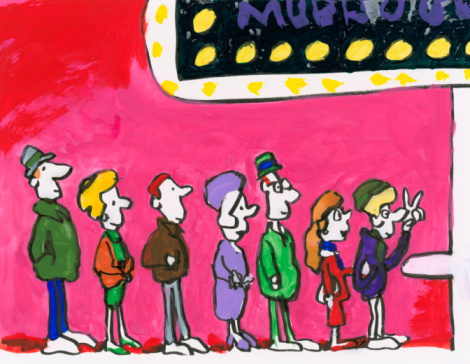
\includegraphics[scale= 0.18]{images/movie.jpg}} \hspace{0.2em}
\onslide<2->{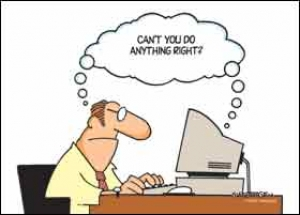
\includegraphics[scale= 0.27]{images/frus.jpg}} \hspace{0.2em}
\onslide<3->{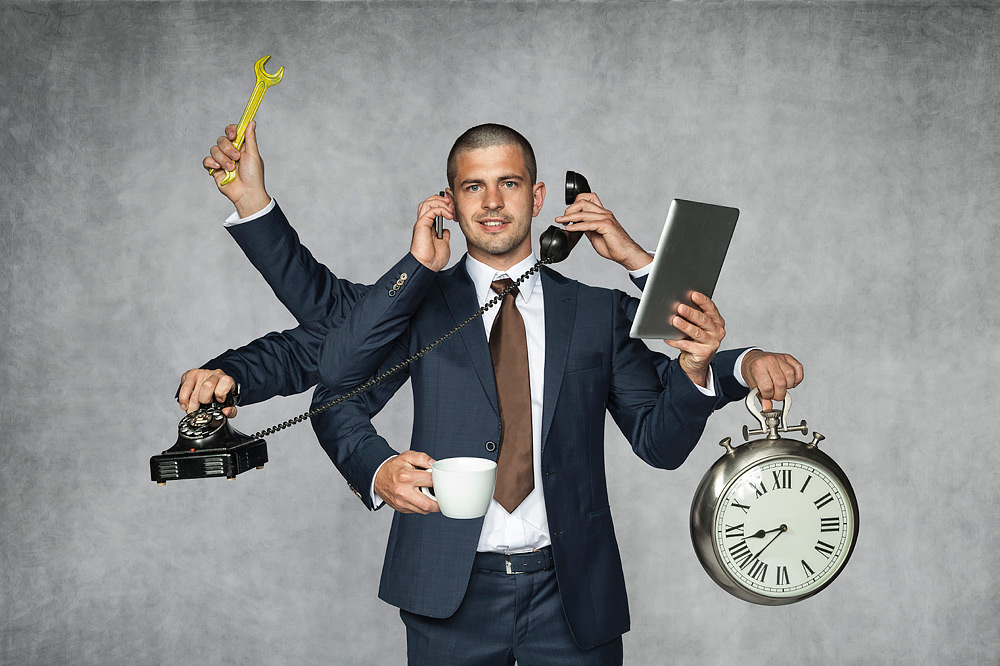
\includegraphics[scale= 0.08]{images/multiple2.jpg}} \hspace{0.2em}
\onslide<4->{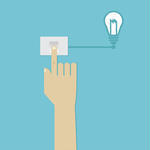
\includegraphics[scale= 1.8]{images/lights.jpg}}\\ \vspace{1.5em}   
\onslide<5->{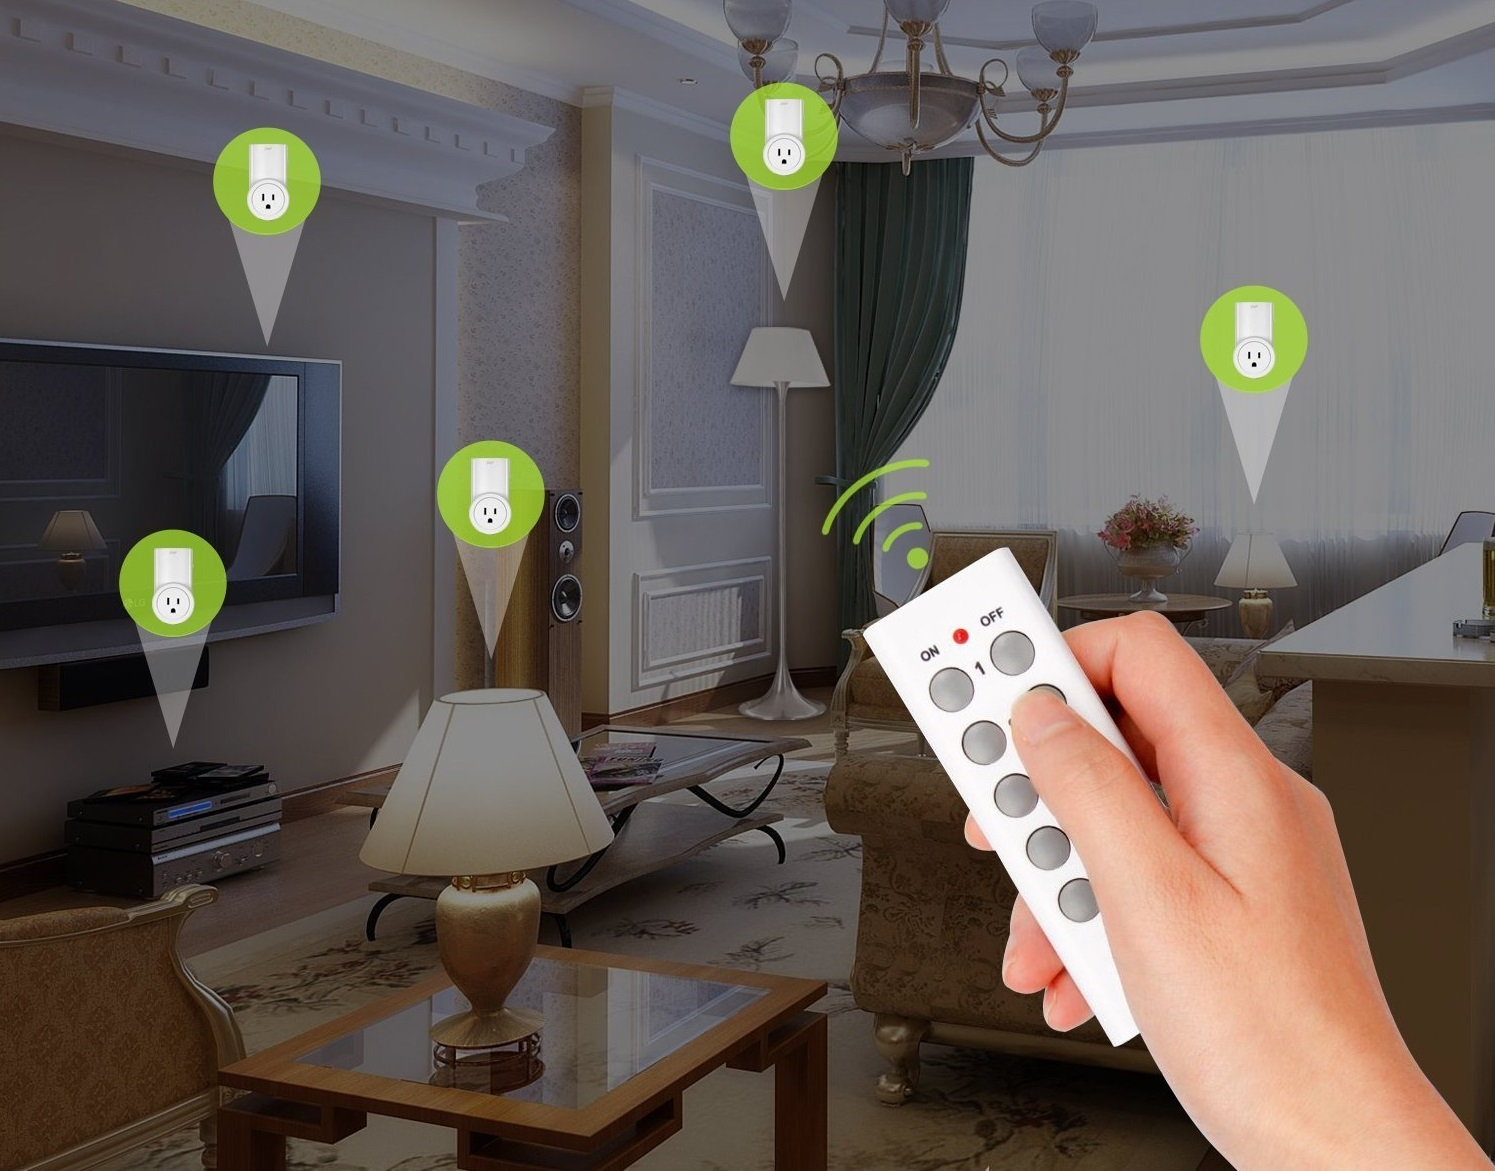
\includegraphics[scale= 0.08]{images/button.jpg}} \hspace{0.2em}
\onslide<6->{
\includegraphics[scale= 0.1]{images/search.jpg}} \hspace{0.2em}
\onslide<7->{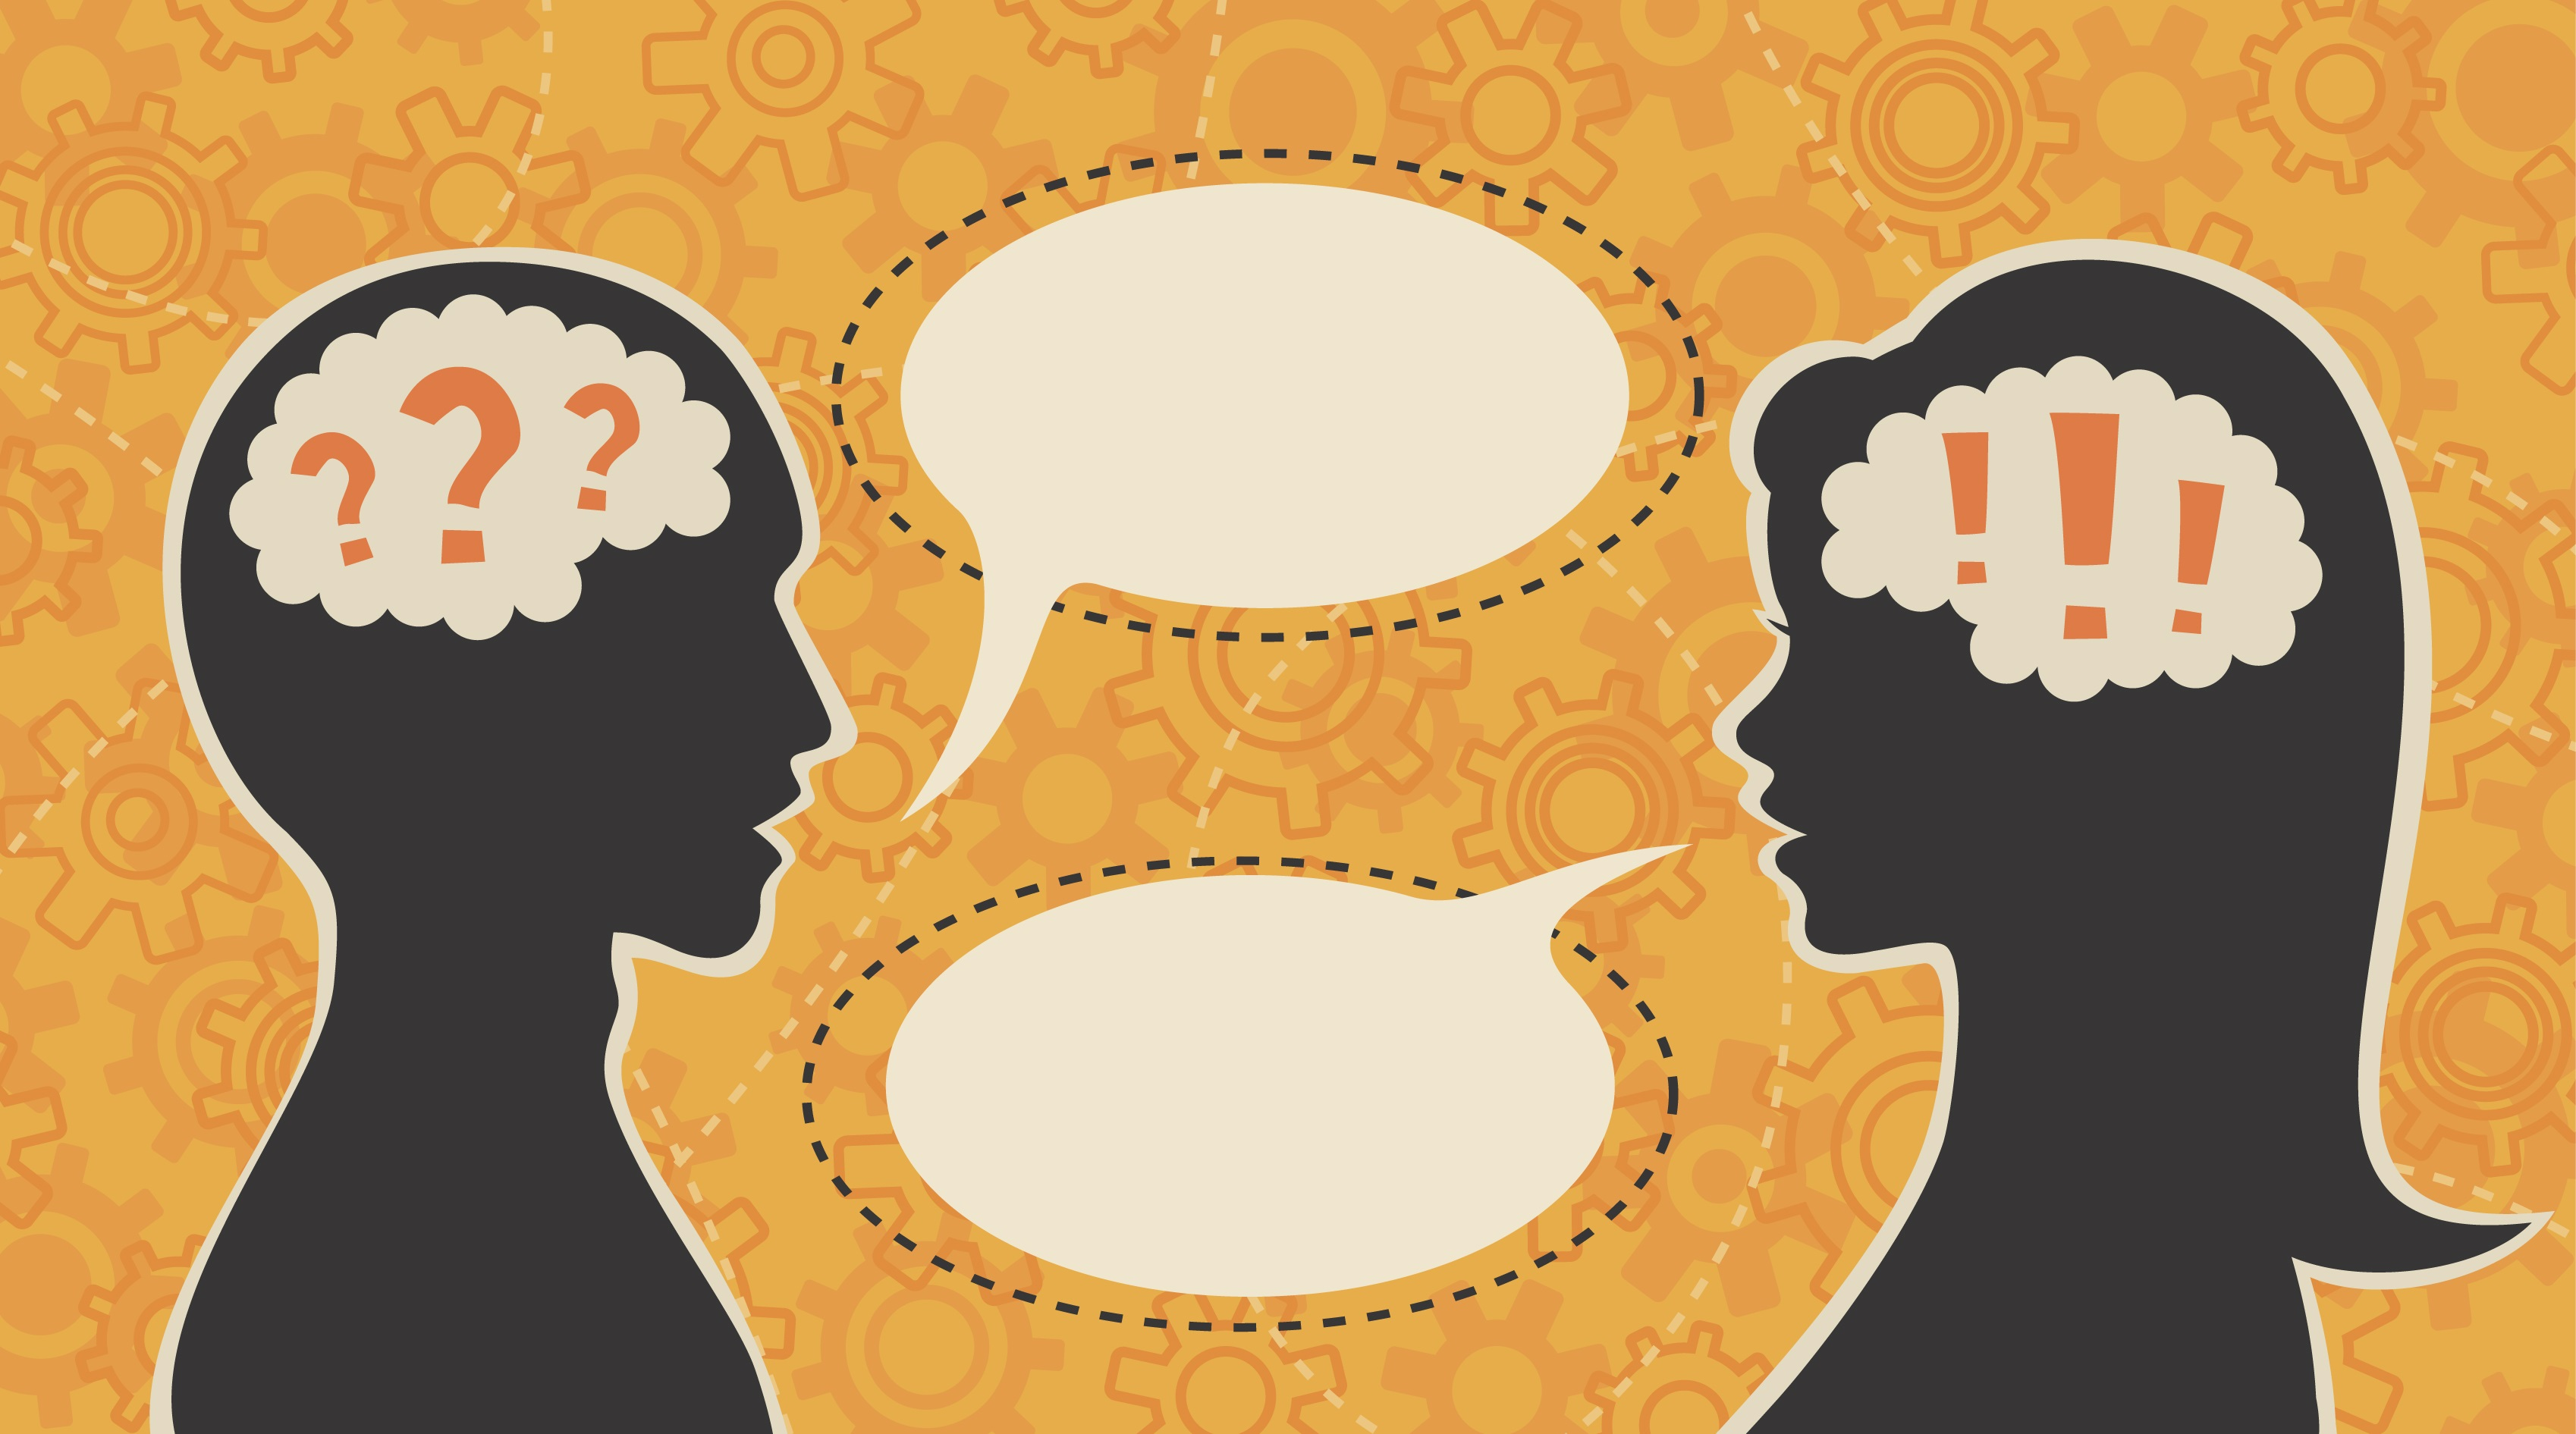
\includegraphics[scale= 0.1]{images/language.jpg}} \hspace{0.2em}
\onslide<8->{
\includegraphics[scale= 0.15]{images/social.jpg}}

\end{figure}
\end{frame}


%------------------------------------------------
\section{Motivation} 
%------------------------------------------------
\begin{frame}
\centering

\includegraphics[scale=0.3]{images/idea.jpg}\\
\vspace{2em}
\textcolor{Blue}{\Huge{\textsf{\textsl{What if we could have one solution to all these problems?}}}}
\end{frame}

\begin{frame}
\frametitle{Motivation}
\begin{figure}
\centering
\resizebox{.6\linewidth}{!}{%
\smartdiagramset{
bubble node size =6cm, 
bubble center node font = \small,
bubble node font = \tiny, 
distance center/other bubbles = 2cm, 
}
\smartdiagramanimated[constellation diagram]{AI Device,Social Network,Intelligent,Answer Basic\\ Questions,Personalized,Connect IOT\\ Devices, Book Tickets,  Identify Images}
}%end resizebox
\end{figure}    
\end{frame}

%------------------------------------------------
\section{Problem Statement}
%------------------------------------------------
\begin{frame} % Need to use the fragile option when verbatim is used in the slide
\frametitle{Problem Statement}
\begin{block}{Statement}
\begin{itemize}
\item To build a Personalised Intelligent Assistant Device that can help humans with the basic task of day to day regimen using their voice.
\item Also to ease the interface of the IOT devices in the surrounding of the Intelligent Device.
\end{itemize}
\end{block}
\end{frame}

%------------------------------------------------
\section{Literature Survey}
%------------------------------------------------
\begin{frame}
\frametitle{Amazon Alexa \small{v/s} \Large{Ivee Sleek} \small{v/s} \Large{Athom Homey}}
\begin{table}
\begin{tabular}{l l l}
\toprule
\textbf{Amazon Alexa} & \textbf{Ivee Sleek} & \textbf{Athom Homey}\\
\midrule
\tiny{Not Open Source} & \tiny{Not Open Source} & \tiny{Not Open Source} \\
\tiny{No efficient android connectivity} & \tiny{No android connectivity} & \tiny{Android connectivity} \\
\tiny{No Connectivity with smart devices}& \tiny{No Connectivity with smart devices}&\tiny{No Connectivity with smart devices}\\
\tiny{No Image Recognition}&\tiny{No Image Recognition}&\tiny{No Image Recognition}\\
\tiny{New features are not integrated}& \tiny{New features are not integrated}&\tiny{New features are not integrated}\\
\tiny{Social Networking can't be integrated}&\tiny{Social Networking can't be integrated}&\tiny{Social Networking can't be integrated}\\
\tiny{Map services are not integrated}&\tiny{Map services are not integrated}&\tiny{Map services are not integrated}\\
\bottomrule
\end{tabular}
\end{table}
\end{frame}

%------------------------------------------------
\section{Introduction}
%------------------------------------------------
\begin{frame}
\begin{center}
\onslide<1->{\textbf{\LARGE{So finally we came up with..!!!}}}\\
\vspace{0.5cm}
\onslide<2->{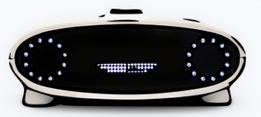
\includegraphics[scale=0.7]{images/mycroft.jpg}}\\
\vspace{0.5cm}
\onslide<3->{\textbf{\LARGE{And we call it}}}
\onslide<4->{\textcolor{Red}{\textbf{\Huge{\hspace{0.5em}{"JASPER"}}}}}
\end{center}
\end{frame}

%------------------------------------------------

\subsection{What is Jasper?}
\begin{frame}[fragile] % Need to use the fragile option when verbatim is used in the slide
\frametitle{What is Jasper?}
\begin{exampleblock}{Introduction}
\begin{itemize}
\item An open source Voice controlled personal assistant device.
\item Written in Python.
\item Built on top of Pocketsphinx STT and Ivona TTS.
\item A standalone intelligent device which can perform basic tasks like Web search, Book Tickets, Integrate mails and many more.
\item Can connect the IOT devices in the vicinity and control them with built-in  voice commands.
\item Connects with a Android app to personalize and control the functionality of the device.
\end{itemize}
\end{exampleblock}
\end{frame}
%------------------------------------------------

\subsection{Why use Jasper?}
\begin{frame}[fragile] % Need to use the fragile option when verbatim is used in the slide
\frametitle{Why use Jasper?}
\begin{exampleblock}{Features}
\begin{itemize}
\item Replace the need of having different devices and application for different task performing.
\item Open to community.
\item Skill sets can be extended.
\item Ease of use through voice commands.
\item Can be personalized.
\item Integrated Android Application.
\item Can interface with IOT devices in the vicinity seamlessly. 
\end{itemize}
\end{exampleblock}
\end{frame}
%------------------------------------------------
%------------------------------------------------
%------------------------------------------------

%----------------------------------------------------------------------------------------
\section{Flow Diagram}
\subsection*{Flow Diagram}
%----------------------------------------------------------------------------------------
\begin{frame}
\frametitle{Flow Diagram}
\begin{center}
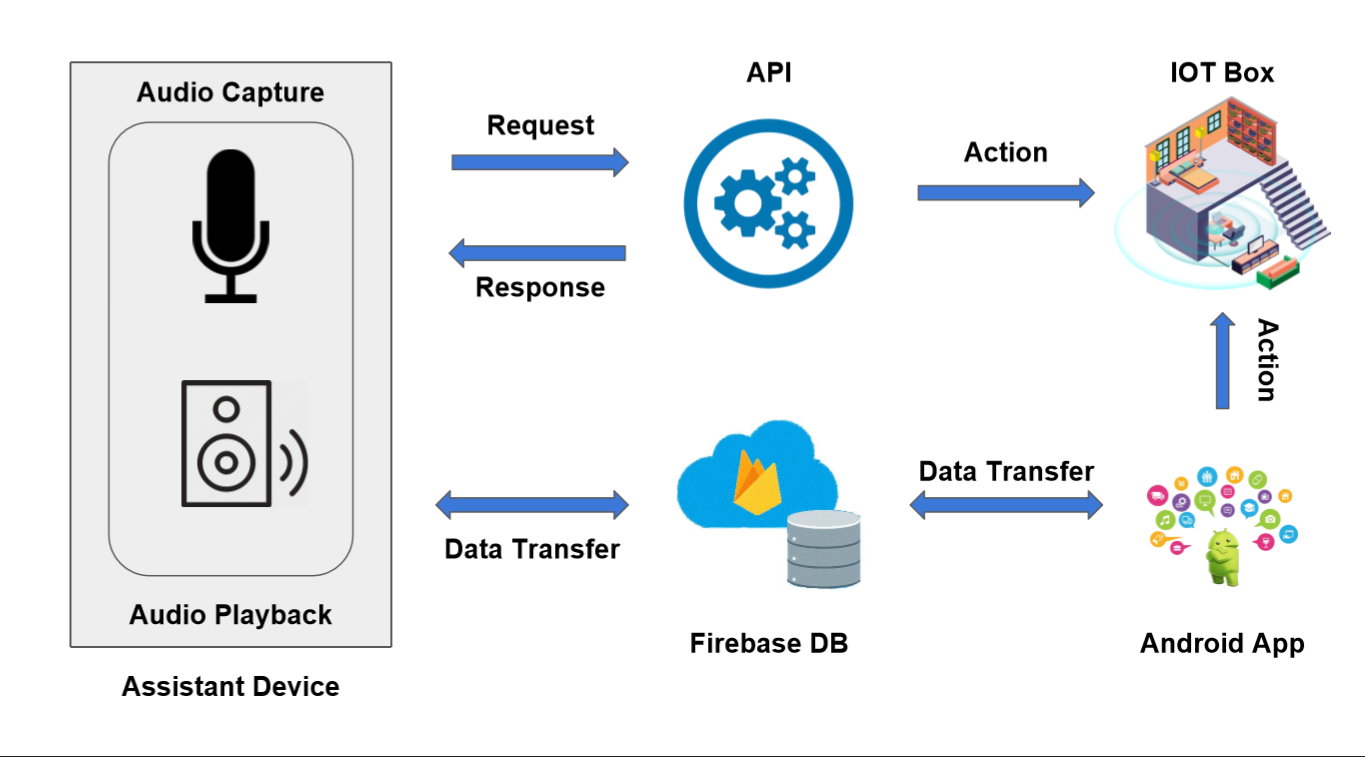
\includegraphics[scale=0.34]{images/Arckin.png}
\end{center}
\end{frame}
%----------------------------------------------------------------------------------------
\subsection*{Detailed Flow Diagram}
%----------------------------------------------------------------------------------------
\begin{frame}
\frametitle{AI Device Flow Diagram}
\begin{minipage}{0.8\textwidth}
\centering 
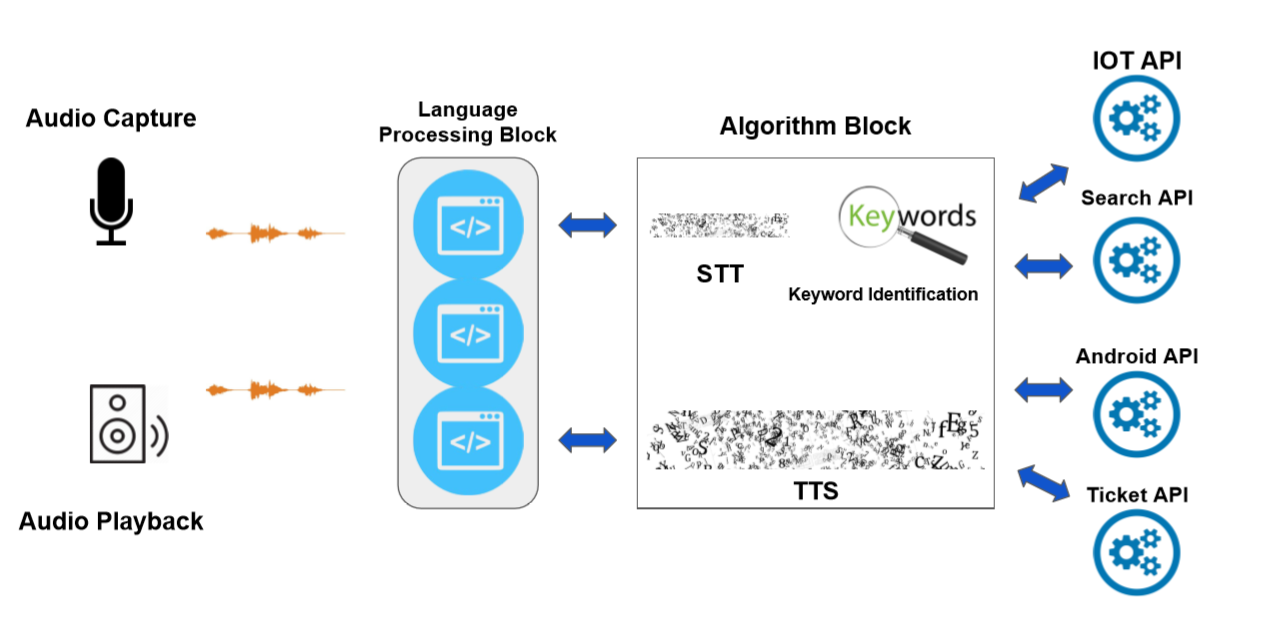
\includegraphics[scale=0.36]{images/Device.png}
\end{minipage}
\end{frame}
%---------------------------------------------------------------------------------------
\begin{frame}
\frametitle{IOT Box Flow Diagram}
\centering
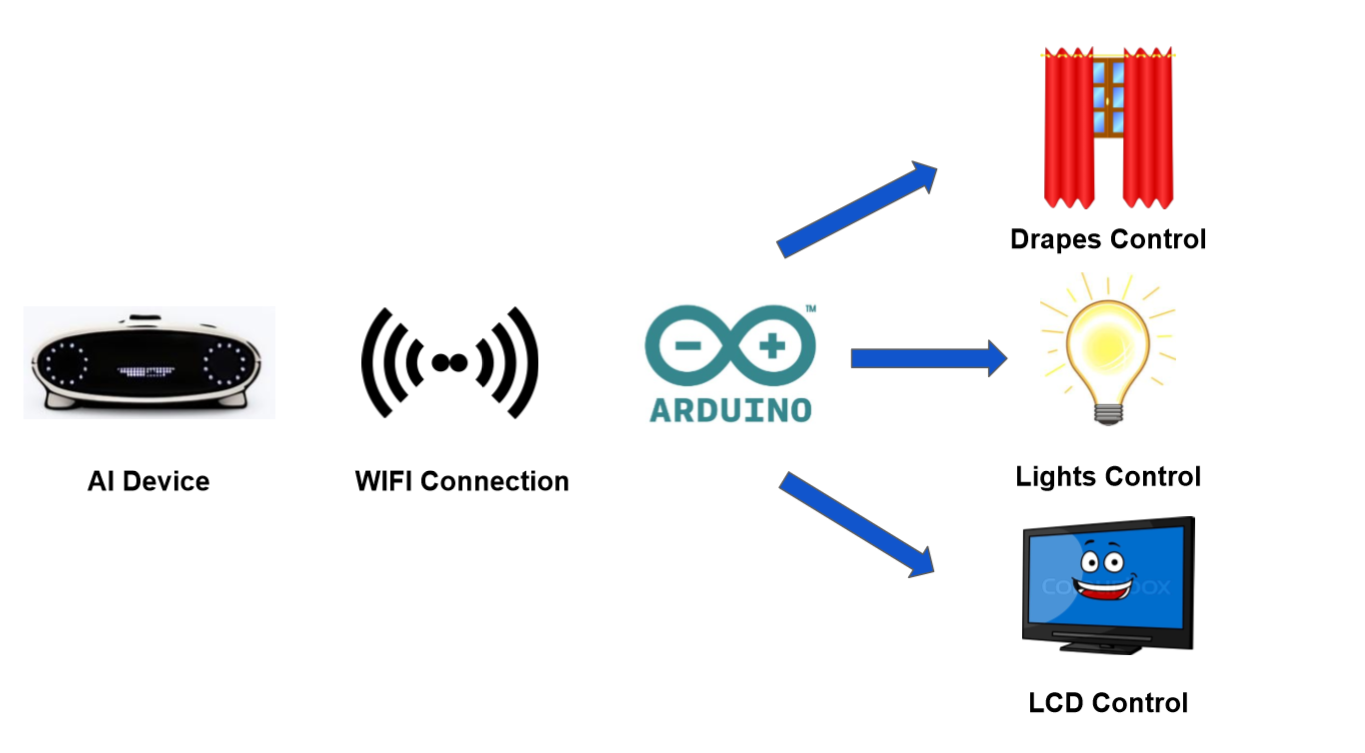
\includegraphics[scale=0.35]{images/IOT.png}
\end{frame}
%----------------------------------------------------------------------------------------
\begin{frame}
\frametitle{Android App Flow Diagram}
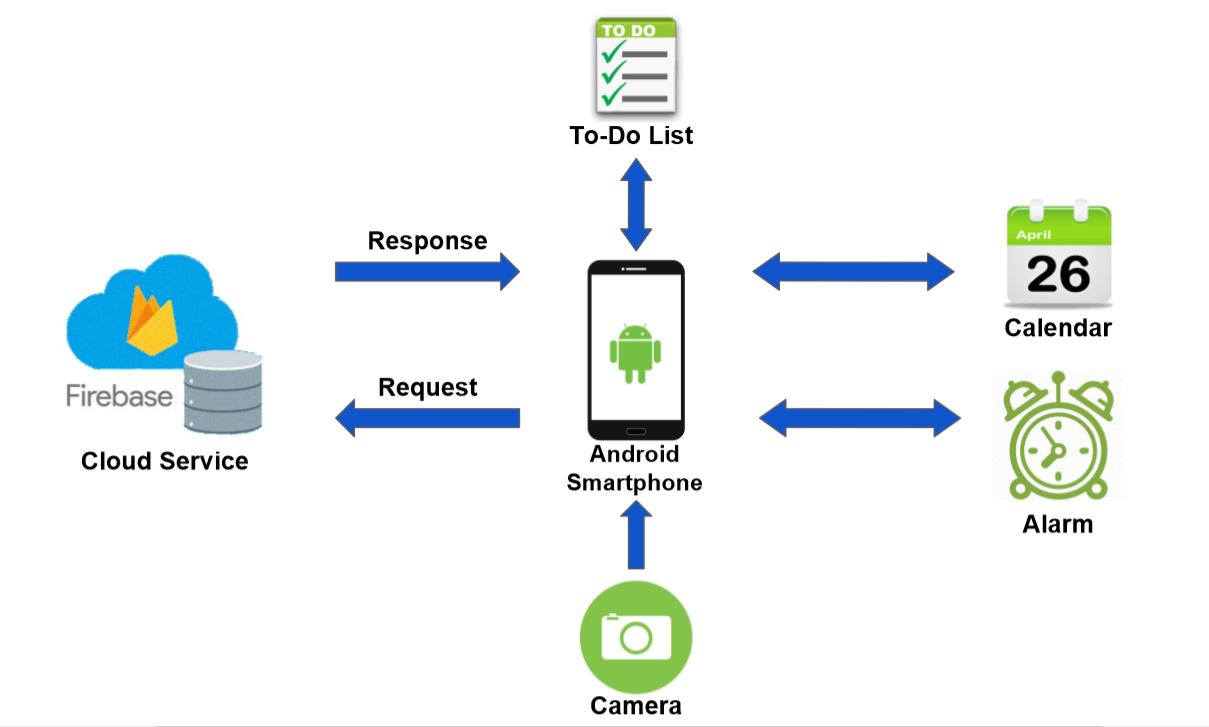
\includegraphics[scale=0.4]{images/android.png}
\end{frame}
%----------------------------------------------------------------------------------------
\section{Key Components}
%----------------------------------------------------------------------------------------
\begin{frame}
\frametitle{Key Components}
The most prominently used software and hardware in Jasper are as follows:
\begin{alertblock}{Key Components}
\begin{itemize}
\item PocketSphinx STT
\item Ivona TTS
\item Firebase Cloud Services
\item Raspberry Pi 3 Model B
\item Arduino Uno
\item Google Translate
\item Scikit Learn
\end{itemize}
\end{alertblock}
\end{frame}
%----------------------------------------------------------------------------------------
\subsection{STT-TTS}
\begin{frame}[fragile]
\frametitle{Key Components}
Following Natural language processing engines will be used in the project:
\begin{columns}[c]
\onslide<1->\column{.45\textwidth} % Left column and width
\begin{exampleblock}{\small{Pocketsphinx STT}}
\begin{itemize}
\item PocketSphinx is a lightweight speaker independent speech recognition engine, specifically tuned for handheld and mobile devices.
\item It is one of the Carnegie Mellon University's open source large vocabulary.
\end{itemize}
\end{exampleblock}

\onslide<2->\column{.45\textwidth} % Right column and width
\begin{exampleblock}{\small{Ivona TTS}}
\begin{itemize}
\item Pyvona is a python wrapper for Amazon’s IVONA. Using Pyvona, great cross-platform text-to-speech is simpler than ever.
\item It is a Open Source TTS built by Amazon and also used in the Amazon Echo.
\end{itemize}

\end{exampleblock}
\end{columns}
\end{frame}
%----------------------------------------------------------------------------------------
\subsection{Pi-Arduino}
\begin{frame}[fragile]
\frametitle{Inverted Index}
Primary hardware which will be used for jasper will be as follows:

\begin{columns}[c]
\onslide<1->\column{.45\textwidth} % Left column and width
\begin{exampleblock}{\small{Raspberry Pi 3}}
\begin{center}
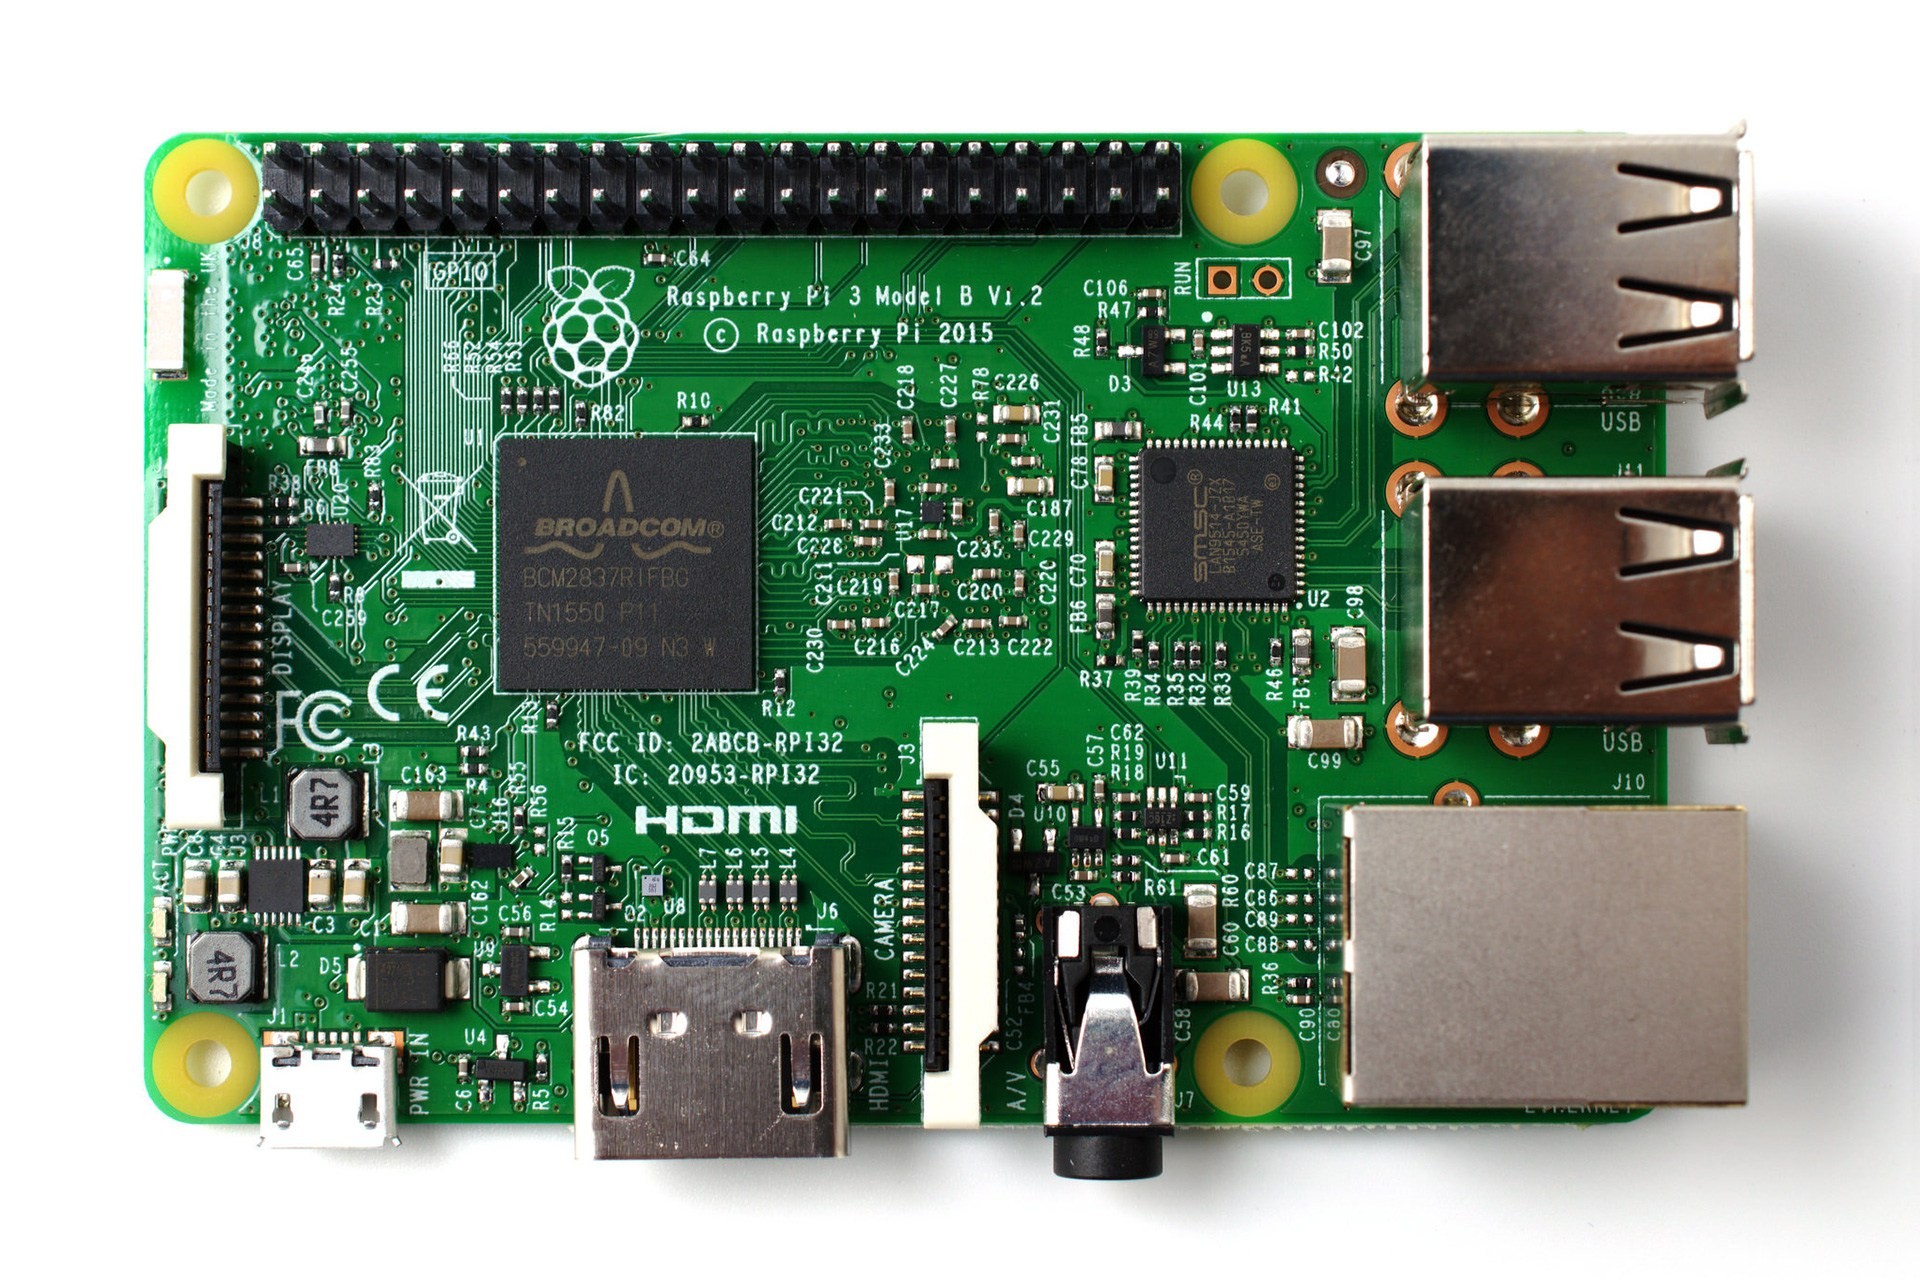
\includegraphics[scale=0.03]{images/pi3.jpg}\\
\begin{itemize}
\item A 1.2GHz 64-bit quad-core ARMv8 CPU
\item 802.11n Wireless LAN
\item Bluetooth 4.1
\item 1GB RAM
\item 40 GPIO Pins
\end{itemize}
\end{center}
\end{exampleblock}

\onslide<2->\column{.45\textwidth} % Right column and width
\begin{exampleblock}{\small{Arduino Uno}}
\begin{center}
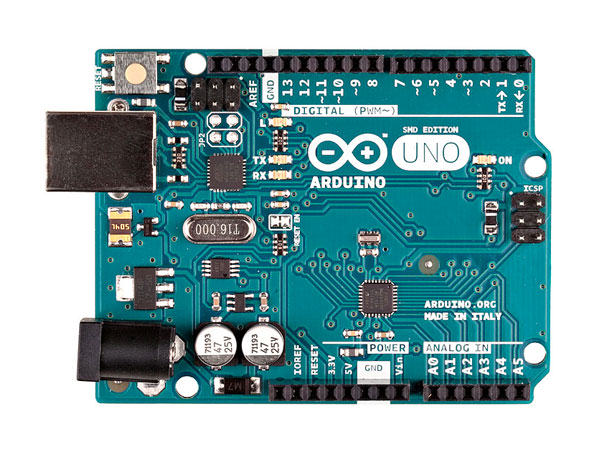
\includegraphics[scale=0.08]{images/arduino.jpg}
\begin{itemize}
\item ATmega328 microcontroller
\item 6 Analog Inputs
\item 32K Flash Memory
\item 14 Digital I/O Pins (6 PWM outputs) 
\end{itemize}
\end{center}
\end{exampleblock}
\end{columns}
\end{frame}
%----------------------------------------------------------------------------------------
\subsection{Firebase-Translate}
\begin{frame}
\begin{columns}[c]
\onslide<1->\column{.45\textwidth} % Left column and width
\begin{exampleblock}{\small{Firebase Cloud Services}}
\begin{center}

\includegraphics[scale=0.1]{images/firebase.png}\\
\end{center}
\small{
Firebase is a cloud services for software developers building mobile or web applications.It provides the following features:
\begin{itemize}
\item Analytics
\item Cloud Messaging
\item Authentication
\item Realtime Database
\item Storage
\item Notifications
\end{itemize}}
\end{exampleblock}

\onslide<2->\column{.45\textwidth} % Right column and width
\begin{exampleblock}{\small{Google Translate}}
\begin{center}

\includegraphics[scale=0.08]{images/google.png}
\end{center}
\small{
\begin{itemize}
\item Google Translate is a free multilingual statistical machine translation service provided by Google to translate text, speech, images from one language into another.
\item Google Translate algorithms are based on statistical analysis rather than traditional rule-based analysis.
\end{itemize}}
\end{exampleblock}
\end{columns}
\end{frame}
%----------------------------------------------------------------------------------------
\section{Advantages}
%----------------------------------------------------------------------------------------
\begin{frame}
 \onslide<1->\frametitle{Advantages}

\resizebox{.8\linewidth}{!}{%
\smartdiagramset{
description title width = 2cm,
description title font = \footnotesize,
description title text width = 2cm , 
description width = 4cm,
description font = \footnotesize ,
descriptive items y sep = 3cm
}
\begin{columns}[T] % align columns
\begin{column}{.48\textwidth}
 \onslide<2->\smartdiagram[descriptive diagram]{
      {\textbf{Open to Community},{Open source and skills can be extended.}},
      {\textbf{Ease-of-Use},{Fully controlled by vocal commands. Can be used by any age group.}},
      {\textbf{Integration of IOT},{IOT Devices in the vicinity can be interfaced using built-in voice commands.}},
      }
\end{column}%
\hspace{2.2cm}%
\begin{column}{.48\textwidth}
 \onslide<3->\smartdiagram[descriptive diagram]{
      {\textbf{Multi-tasking},{Have the capability to perform various types of task, not performed by other voice controlled devices.}},
      {\textbf{Personalized},{Features like mail integration, To-do list and many more}},
      {\textbf{Out-of-box Features},{Features like Image recognition, Android app and One Device multiple Social Networks.}},
      }
\end{column}%
\end{columns}}
\end{frame}
%----------------------------------------------------------------------------------------
\section{Conclusion}
%----------------------------------------------------------------------------------------
\begin{frame}
\frametitle{Conclusion}
\openup 0.7em

Jasper is a \textbf{Step Forward} to the era of Voice controlled Personal Assistant Device.\\ It is a great \textbf{Open Source Platform} built on top of Open source NLP tools and still performs according to the like of other alternative present.\\ Also it is \textbf{easy to setup} and \textbf{get started} with.\\ And it also supports on go \textbf{integration of IOT devices} which other Personal assistant devices does not, with an \textbf{Android app} built on top of it. 

\end{frame}
%----------------------------------------------------------------------------------------
\section{Future Scope}
%----------------------------------------------------------------------------------------
\begin{frame}
\frametitle{Future Scope}
\begin{alertblock}{Future Scope}
\begin{itemize}
\item The device can make a conversation with the user instead of just servicing the commands.
\item Language translation on go for multiple languages.
\item More than one jasper can connect to form a web of Personal Assistant Devices.
\item Making Phone calls and voice mails integration using the AI Device. 
\end{itemize}
\end{alertblock}
\end{frame}
%----------------------------------------------------------------------------------------
\section{References}
%----------------------------------------------------------------------------------------
\begin{frame}
\frametitle{References}
\begin{thebibliography}{5}
\bibitem{beamer} \emph{ Nil Goksel-Canbek ,Mehmet Emin Mutlu: On the track of Artificial Intelligence: Learning with Intelligent Personal Assistants , 2016.}{\vspace{.6cm}}
\bibitem{beamer2} \emph{Harshita Phatnani, Mr. Jyotiprakash Patra, Ankit Sharma: An Intelligent Voice Assistant Using Android Platform , 2016 }{\vspace{.6cm}}
\bibitem{beamer2} \emph{Vinay Sagar, Kusuma SM:Home Automation Using IOT , 2015 }{\vspace{.6cm}}
\bibitem{beamer2} \emph{ Douglas OShaughnessy, Senior Member: Interacting With Computers by Voice: Automatic Speech Recognition and Synthesis,2003}{\vspace{1cm}}
\end{thebibliography}
\end{frame}
%----------------------------------------------------------------------------------------
\begin{frame}
\begin{center}
\textbf{\huge{Thank You!!!}}\\
\vspace{0.5cm}

\includegraphics[scale=3]{images/thanks.png}
\\\vspace{0.5cm}
\textbf{\textsl{\huge{Questions?}}}\\
\end{center}
\end{frame}
%----------------------------------------------------------------------------------------
\end{document} 
